 \documentclass[12pt]{article}
\usepackage[a4paper, margin=.30in]{geometry}

\usepackage{array}
\usepackage{graphicx, subfig, wrapfig, fancyhdr, lastpage }
\newcommand\headerMe[2]{\noindent{}#1\hfill#2}
\usepackage[mathscr]{euscript}



\pagestyle{fancy}
\fancyhf{}

\rfoot{\em{Page \thepage \hspace{1pt} / \pageref{LastPage}}}
\begin{document}

\headerMe{Royaume du Maroc}{année scolaire \emph{2024-2025}}\\
\headerMe{Ministère de l'Éducation nationale, }{  Professeur :\emph{Zakaria Haouzan}}\\
\headerMe{du Préscolaire et des Sports}{Établissement : \emph{Lycée SKHOR qualifiant}}\\

\begin{center}
Devoir  N°1 \\
   Filière Tronc Commun Scientifique\\
Durée 1h30
\\
    \vspace{.2cm}
\hrulefill
\Large{Chimie 7pts}
\hrulefill\\

    %\emph{Les Trois parties sont indépendantes}
\end{center}
%end Headerss------------------------
 \section*{Partie 1 :Classification périodique des éléments chimiques \dotfill (7pts) }
Un élément X se trouve dans la 3 ème période et dans le groupe (II) du tableau périodique simplifiée.
\begin{enumerate}
    \item Déterminer la structure électronique de l'atome de l'élément X.\dotfill(1pt)

    \item Déterminer le numéro atomique de cet élément ainsi que son symbole et son nom. \dotfill(1pt)
    \item Nommer la famille à laquelle cet élément chimique appartient.\dotfill(1pts)
    \item Citer un autre éléments appartenant à la même famille.\dotfill(1pt)
 \item Quel ion monoatomique est susceptible de se former à partir de l’atome cet élément ?\dotfill(1pt)
 \item Quel est le nombre d'électrons de valence que possède l’atome X ?\dotfill(1pt)
 \item Quel est le nombre totale d'électrons que possède l’atome X?\dotfill(1pt)
\end{enumerate}
%__________________Chimie ______________________-
%%%%%%%+_+_+_+_+_+_+_+_+_Partie1

%_____________________________________PHYSIque Partie 22222____________________________________________________________________________
\begin{center}
    %\vspace{2cm}
\hrulefill
\Large{Physique 13pts}
\hrulefill\\
    \emph{Les deux parties sont indépendantes}
\end{center}
%end Headerss------------------------

 \section*{Partie 1 :Équilibre d’un corps solide soumis à trois forces non parallèles (7 pts)}

\begin{wrapfigure}[5]{r}{0.36\textwidth}
    \vspace{-1.8cm}
    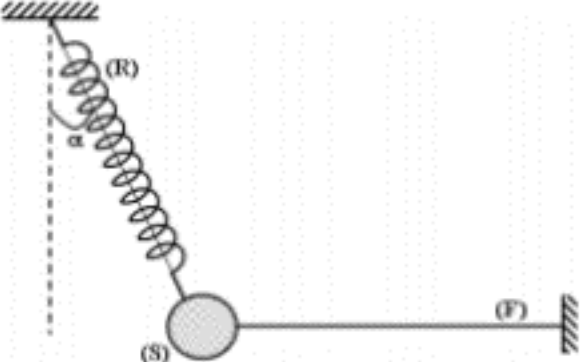
\includegraphics[width=0.36\textwidth]{./img/pendule_simple.png}
\end{wrapfigure}

On considère un solide (S) de masse
m=200g, accroché à un ressort (R) et à un fil (F) d'intensité F = 1.2N comme l’indique la figure ci-contre.

Le ressort de raideur K=40N/m est
incliné d’un angle $\alpha$=30° par rapport à la
verticale. Le fil est horizontal. On prendra g=10N/Kg.

\begin{enumerate}
    \item Faire le bilan des forces qui
s’exercent sur le solide (S) et les
        représenter sur la figure.\dotfill(1pt)

    \item Ecrire la condition de l’équilibre du solide (S).\dotfill(1pt)
    \item Donner les expressions des coordonnées de chacune des forces dans le repére $(O, x, y)$ en fonction de leurs intensités.\dotfill(1pts)
    \item Déterminer la tension T du ressort : \dotfill(2pt)
        \begin{enumerate}
            \item Par méthode analytique.
            \item Par méthode géométrique en utilisant une échelle convenable
        \end{enumerate}
    \item déduire l’allongement du ressort.\dotfill(1pt)
    \item déterminer la longueur finale L du ressort à l’équilibre sachant que sa longueur initiale est L0 = 20 cm \dotfill(1pt)
\end{enumerate}

\vspace{3cm}

\hrulefill\\
%_________________partie 2  : gravitation universelle :)
\section*{Partie 2 :La poussée d'Archimède exercée sur un pavé \dotfill(2 pts)}
Un pavé flotte à la surface de l’eau. Ses dimensions sont : $h = 20 cm$ ,  $L = 60 cm$ ,  $l = 20 cm$.

\begin{wrapfigure}{r}{0.38\textwidth}
	\vspace{-4.3cm}

	
 \begin{center}
	 \hspace{-3cm}	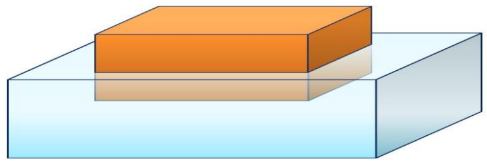
\includegraphics[width=0.38\textwidth]{./img/img01.png}
\end{center}
\end{wrapfigure}
\begin{enumerate}
	\item  Le pavé émerge sur une hauteur de $h' = 17 cm$. Calculer le volume V' de la partie immergée.\dotfill{0,25pts}

	\item  Calculer la masse $m'_{dep}$ d’eau déplacée.\dotfill{0,25pts}
	\item  Calculer le poids $P'_{dep}$ d’eau déplacé.\dotfill{0,25pts}
	\item  déduire la valeur du poids P du pavé.\dotfill{0,25pts}
	\item  Préciser le matériau constituant ce pavé.\dotfill{1pt}
\end{enumerate}

\textbf{Donnée: } La masse volumique d'eau: $\rho_{eau} = 1000 kg/m^3$ , L'intensité de pesanteur: $g = 10N/kg$.

\begin{center}
\begin{tabular}{ |c| c| c| c|c|c| }
	\hline
	\textbf{Matériau}                   & Polystyrène & Bois &glace &Aluminium&Fer\\\hline 
	\textbf{Masse volumique} $(kg/m^3)$ & 11 & 850 &920 &2700& 8000\\\hline
\end{tabular}
\end{center}

\section*{Partie 3 : Equilibre d'un solide\dotfill(4 pts)}
Un solide ( S ) de masse $m = 200 g$ est maintenue à l’équilibre sur un plan incliné parfaitement lisse
d’inclinaison $\alpha = 30^{\circ}$ par rapport à l’horizontale par l’intermédiaire d’un ressort de masse négligeable , de
constante de raideur $k = 40 N.m^{-1}$ et allongé . L’axe du
ressort fait un angle $\theta= 20^{\circ}$ avec la ligne de la grande
pente du plan incliné.

\begin{enumerate}
  
	\item  Rappeler la condition d’équilibre d’un solide soumis à trois forces.\dotfill{1pts}
 \item Donner les expressions des coordonnées de chacune des forces dans le repére $(O, x, y)$ en fonction de leurs intensités.\dotfill(1pts)
 \item Exprimer l’allongement $\Delta$L du ressort en fonction de $m, g, \theta, K$ et $\alpha$ \dotfill(1pts)
 \item Calculer $\Delta$L\dotfill(1pts)
\end{enumerate}

\textbf{Donnée: }  L'intensité de pesanteur: $g = 10N/kg$.
 \begin{center}
	 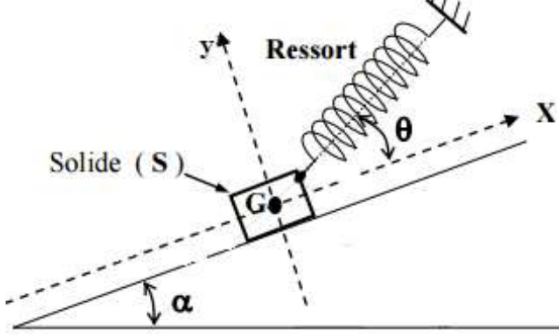
\includegraphics[width=0.4\textwidth]{./img/img02.png}
\end{center}


\end{document}
